\scanpage{46}\mspage{45}
to define a figure $F'$ as a \uline{\unsure{refinement|refinement}} of $F$, if each $X'\in F'$ \deleted{\unsure{déf}} is a refinement of an $X\in F$. So it is better to take as primitive notion that of \uline{subdivision} of a \deleted{\unsure{mul}} \inserted{figure}, (which will reduce ; that of a multistratum), and define a refinement of a figure as a subfigure of a subdivision.

So, new start !

A country $C$ is defined by a triple
\[
 (M,\mathcal F,\Sigma)
\]
where $ M$ is a set (set of \uline{multistrata}), $\mathcal F$ a set of subsets of $ M$ ($\mathcal F\in\mathcal P(\mathcal P(M))$), \inserted{\unsure{called|called} \uline{figures},} and $\Sigma$ a relation on $\mathcal F$ called : $F'$ \uline{subdivides} $F$. \unsure{Axioms|Axiom}
% slanted
\margin{If $F\in\mathcal F$, the $X\in F$ are the (multi)strata of $F$}

\uline{C 1} For every $X\in M$, $\exists$ \unsure{a|a} smallest \deleted{subset} figure \deleted{which} $F_X\unsure{\subset|{,}}$ such that $X\in F$.

It is called the \uline{elementary figure} defined by $X$. We write
\[
 X\leq Y\ \overset{\mathrm{def}}{\Longleftrightarrow}\ F_X\subset F_Y\qquad\text{i.e. }X\in F_Y
\]
and we find an \uline{order}$^{*}$ relation $\leq$ on $ M$.\textsuperscript{$*$}
\margin{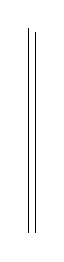
\begin{tikzpicture}\draw (0,0)--(0,2.6);\draw (.09,0)--(.09,2.55);\end{tikzpicture}}
% slanted
\margin{$^{*}$ We want this to be an order relation and not merely a preorder relation, i.e. \uline{C$'$1} if \deleted{\unsure{pr}} $X\ne Y$, $\exists$ $F\in\mathcal F$ which \unsure{contains} one of the two \unsure{multistrata} $X,Y$, and not the other, i.e. $F_X\ne F_Y$.}
% slanted
\margin{-- i.e. $\mathcal F$ \unsure{separated|separates} the elements of $ M$}
